\documentclass[12pt,a4paper]{article}
\usepackage[utf8]{inputenc} %polskie znaki
\usepackage[T1]{fontenc}	%polskie znaki
\usepackage{amsmath}		%matematyczne znaczki :3
\usepackage{enumerate}		%Dodatkowe opcje do funkcji enumerate
\usepackage{geometry} 		%Ustawianie marginesow
\usepackage{graphicx}		%Grafika
\usepackage{wrapfig}		%Grafika obok textu
\usepackage{float}			%Allows H in fugire
\pagestyle{empty} 			%usuwa nr strony

\newgeometry{tmargin=2cm, bmargin=2cm, lmargin=2cm, rmargin=2cm} 

\begin{document}
			\begin{center}
		\LARGE Planimetria - powtórka przed sprawdzianem
	\end{center}
	\vspace{1.5cm}
	\begin{tabular}{p{13cm} r}
		Imię i nazwisko: ............................................................................
	 &[....../30pkt]\\ 
	 \vspace{0.5cm}
	\end{tabular}
	\begin{enumerate}[1.]
		\item  \begin{tabular}{p{13cm} r}
			Oblicz "x" i "y" &[3pkt]\\ 
		\end{tabular}
	\begin{figure}[h]
		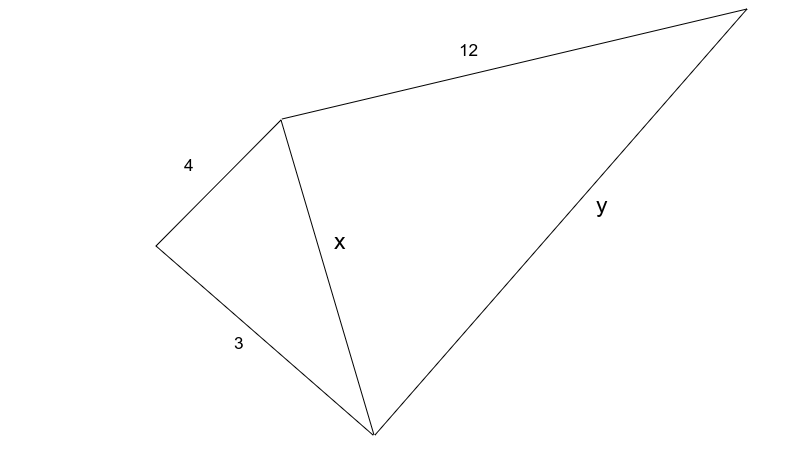
\includegraphics[scale=0.4]{p1}
	\end{figure}
		\item  \begin{tabular}{p{13cm} r}
			Oblicz kąty $\alpha$, $\beta$, $\gamma$, $\delta$ &[5pkt]\\ 
		\end{tabular}
	\begin{figure}[h]
		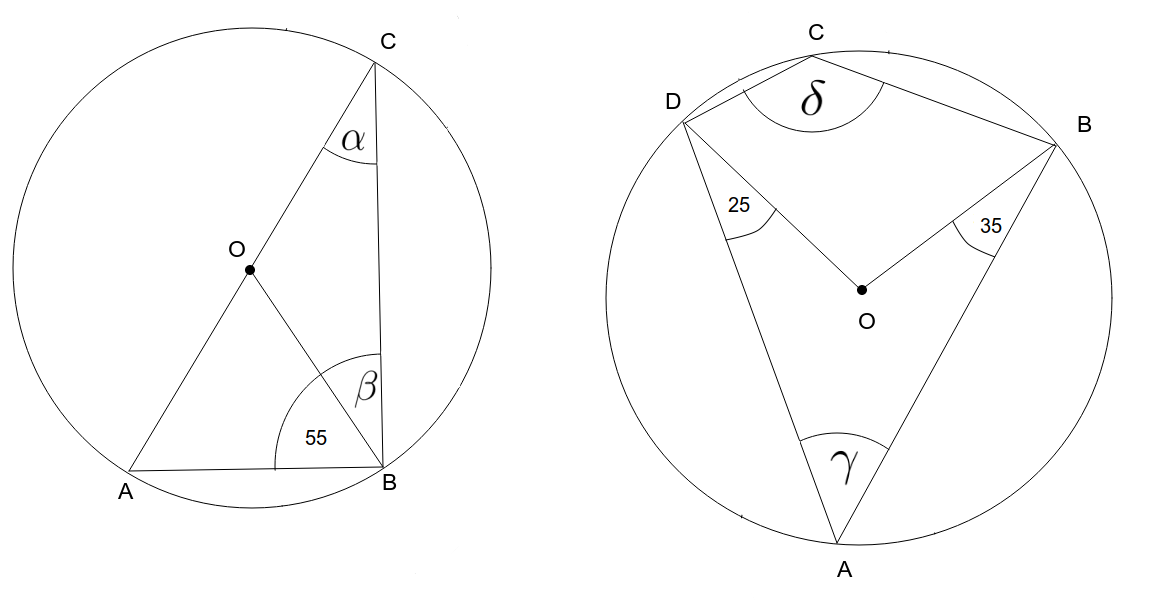
\includegraphics[scale=0.4]{p2}
	\end{figure}
		\item  \begin{tabular}{p{13cm} r}
			W pewnym prostokącie jeden z tego boków jest o 4 większy od drugiego. Wiedząc, że przekątna tego prostokąta wynosi $2\sqrt{10}$, oblicz jego obwód.&[4pkt]\\ 
		\end{tabular}
	\newpage
		\item  \begin{tabular}{p{13cm} r}
			Oblicz obwód i pole trapezu równoramiennego: &[4pkt]\\ 
		\end{tabular}
	\begin{figure}[h]
		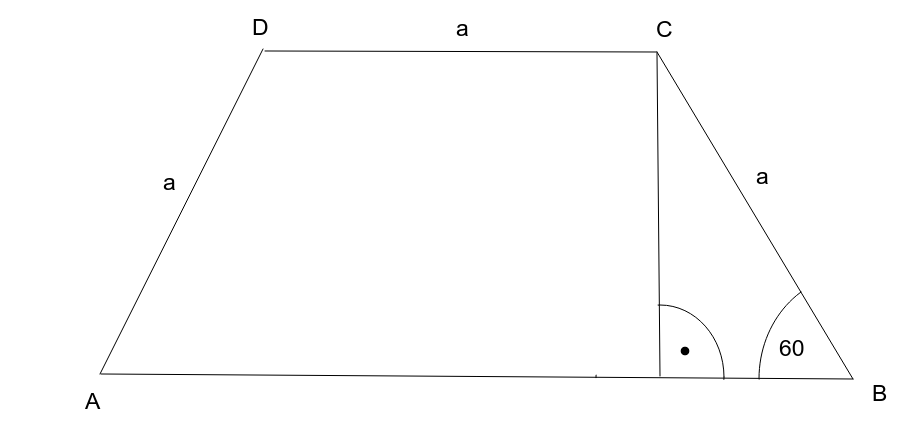
\includegraphics[scale=0.6]{p3}
	\end{figure}
		\item  \begin{tabular}{p{13cm} r}
			Dany jest trójkąt równoramienny o podstawie długości 10 i wysokości 12. Oblicz promień okręgu wpisanego w ten trójkąt. &[4pkt]\\ 
		\end{tabular}
		\item  \begin{tabular}{p{13cm} r}
			Dany jest trapez o ramionach długości 17 i $4\sqrt{5}$ oraz podstawach długości 5 i 24. Oblicz wysokość tego trapezu. &[5pkt]\\ 
		\end{tabular}
		\item  \begin{tabular}{p{13cm} r}
			Dany jest trójkąt równoramienny, którego stosunek długości ramienia do podstawy wynosi 3:2. Oblicz obwód tego trójkąta wiedząc, że jego pole wynosi $18\sqrt{2}$. &[5pkt]\\ 
		\end{tabular}
	\end{enumerate}
\end{document}